\documentclass[journal]{IEEEtran}
\usepackage[T1]{fontenc}
\usepackage[utf8]{inputenc}
\usepackage{amsmath,amssymb,bm}
\usepackage{fix-cm}
\usepackage{graphicx,booktabs,array,multirow}
\usepackage{cite,microtype,xurl}
\usepackage[hidelinks]{hyperref}
\usepackage{placeins}
\newcommand{\method}{\textsc{AnyGSLoc}}
\graphicspath{{figures/}}
\hyphenation{local-iza-tion land-mark land-marks Gauss-ian Super-Point repro-jection}
\hypersetup{pdftitle={AnyGSLoc: From Gaussian Splatting to Localization Maps},pdfauthor={}}
\setlength{\textfloatsep}{9pt plus 2pt minus 2pt}
\setlength{\dbltextfloatsep}{10pt plus 2pt minus 2pt}
\setlength{\floatsep}{8pt plus 2pt minus 2pt}
\setlength{\dblfloatsep}{9pt plus 2pt minus 2pt}
\setcounter{topnumber}{2}
\setcounter{dbltopnumber}{1}
\renewcommand{\topfraction}{0.90}
\renewcommand{\dbltopfraction}{0.85}
\renewcommand{\textfraction}{0.10}
\raggedbottom
\newcommand{\tabnote}[1]{\par\smallskip\begin{minipage}{\linewidth}\footnotesize #1\end{minipage}}

\newcounter{anygsalgorithm}

% Accepted experiments integrated 2026-10-13. Values refer to T1/T4/T7/T8.
\newcommand{\numScenes}{24}
\newcommand{\numQueries}{24,700}
\newcommand{\numPriors}{seven}
% Production Full; Cambridge scene-equal mean of scene medians.
\newcommand{\numCamTE}{7.82}
\newcommand{\numCamRE}{0.12}
\newcommand{\numCamRfive}{46.95}
\newcommand{\numFullStorage}{585.69}
\newcommand{\numFullTime}{77.22}
% Production Compact; distinct from Full.
\newcommand{\numCompactTE}{8.54}
\newcommand{\numCompactRE}{0.12}
\newcommand{\numCompactStorage}{126.73}
\newcommand{\numCompactTime}{74.19}
\newcommand{\numCompression}{78.36}
% Current T5 3DGS shared-observation mapping-view diagnostic (Fig. E2).
\newcommand{\numResTrack}{0.68}
\newcommand{\numResDepth}{17.32}
\newcommand{\numResCenter}{4.92}


\title{AnyGSLoc: From Gaussian Splatting to Visual Localization Maps}
\author{}
\begin{document}
\maketitle
\begin{abstract}
We study how a prebuilt Gaussian scene can be converted into an explicit map for visual relocalization. AnyGSLoc uses Gaussian rendering only to obtain offline reference observations; multiview feature tracks then determine the 3D landmarks and their descriptors independently of Gaussian primitive identities. Rendering-aware observation filtering controls the evidence entering association, robust triangulation recovers landmark positions, and view-balanced fusion represents their appearance. A localization-aware selector retains landmarks that jointly provide reliable, well-covered, and complementary pose constraints. The resulting map requires no original mapping images or scene-specific feature training and supports direct 2D--3D localization without online rendering. Experiments cover 24 indoor and outdoor scenes and seven Gaussian model configurations. On Cambridge, Compact achieves 8.54\,cm/$0.12^\circ$ average scene-median error at 74.19\,ms localization time. Relative to the Full candidate bank, it removes 78.36\% of the landmarks and reduces five-scene storage from 585.69 to 126.73\,MB, while average scene-median translation error changes from 7.82 to 8.54\,cm.
\end{abstract}
\begin{IEEEkeywords}
Visual localization, Gaussian splatting, map construction, multiview geometry, landmark selection.
\end{IEEEkeywords}
\section{Introduction}
\label{sec:introduction}
Visual relocalization recovers the pose of a camera with respect to a previously mapped environment. A common solution is structure-based localization: image features are matched to 3D landmarks and the pose is recovered from the resulting 2D--3D correspondences~\cite{sarlin2019hloc,lepetit2009epnp}. The effectiveness of this formulation depends on a simple property of the map: a stored landmark should represent the image evidence that will be matched at query time, and its 3D position should be consistent with that evidence.

\begin{figure}[!t]
\centering
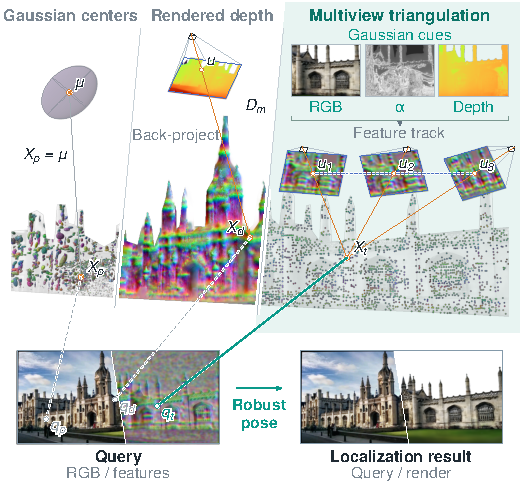
\includegraphics[width=\linewidth]{Fig1_geometry_to_localization.pdf}
\caption{From a Gaussian scene to a localization map. Gaussian centers and back-projected depth provide coordinate alternatives; our map triangulates multiview feature tracks. The lower panels show a query correspondence and alignment at the estimated Compact-map pose. Rendering visualizes the result and is not part of query localization.}
\label{fig:fig1}
\end{figure}


3D Gaussian Splatting (3DGS) has become a practical representation for reconstructing and rendering scenes~\cite{kerbl2023gaussian,huang2024_2dgs,guedon2025matcha}. This creates an appealing opportunity for localization: once a Gaussian scene is available, reference observations can be rendered from it instead of maintaining a separate localization map-building pipeline. The difficulty is that a rendering primitive is designed to contribute to image synthesis, whereas a localization landmark is used to explain a feature correspondence. These are related roles, but they do not require the same geometric representation. A Gaussian center is tied to a primitive rather than to a particular image feature, while a rendered depth value inherits the renderer's view-dependent depth assignment.

This distinction matters when a Gaussian scene is converted into an explicit localization map. The coordinate attached to a matched feature should be supported by the pixels that identify the same scene element across views. In other words, the rendering model should provide observations, while the observations themselves should determine the localization landmarks. This perspective keeps the geometric role of the Gaussian scene and that of the localization map separate without discarding the useful information provided by rendering.

\method{} follows this principle by constructing landmarks from multiview feature tracks on rendered reference views. Each track establishes which pixels correspond to one scene feature; calibrated rays from those pixels then determine a 3D position, and the same observations provide the landmark descriptor. Rendering is therefore used as an offline source of observations and geometric cues, not as the definition of the exported landmark. Figure~\ref{fig:fig1} summarizes this separation.

A second issue is that not every rendered observation is equally useful for correspondence construction. Local rendering artifacts, weak geometric support, and visually uninformative regions can produce detections that are distinctive but unreliable. We therefore filter observations before cross-view association, construct tracks using descriptor similarity together with epipolar geometry, and recover additional associations with rendered depth where the sparse camera graph leaves gaps. The resulting tracks are converted into landmarks by robust triangulation and view-balanced descriptor fusion. Finally, a localization-aware selector retains a compact subset by considering landmark quality, reference-view support, and the pose constraints supplied by the selected map.

The resulting system has a deliberately simple online interface. After offline construction, only landmark coordinates and descriptors are required. A query is matched directly to the compact 3D landmark map and localized with a robust pose solver, with no Gaussian rendering, image retrieval, or separate dense refinement at inference time. Thus the Gaussian scene remains the source of the map, while the deployed localization representation is an explicit, compact correspondence map.

The contributions are threefold:
\begin{enumerate}
\item \textit{Track-based landmark construction from Gaussian scenes.} We establish a correspondence-grounded conversion from a prebuilt Gaussian scene to an explicit localization map. Feature tracks, rather than Gaussian primitive identities, determine landmark geometry and appearance, with multiview triangulation providing the exported 3D coordinates.
\item \textit{Reliable observation and appearance construction.} We introduce a rendering-aware observation filtering procedure before association and a view-balanced multiview descriptor fusion scheme after tracking. Together they suppress unreliable rendered observations while preventing densely sampled viewpoints from dominating a landmark descriptor.
\item \textit{Localization-aware map selection.} We compact the reconstructed landmark bank by combining quality pruning, reference-view coverage completion, and pose-aware completion. The final map preserves complementary localization constraints while substantially reducing the deployed representation.
\end{enumerate}

We evaluate the resulting Compact map on \numScenes{} indoor and outdoor scenes and use the complete candidate bank, Full, to isolate the effect of selection. On Cambridge, Compact achieves $\numCompactTE\,cm/\numCompactRE^\circ$ average scene-median error with \numCompactStorage{}\,MB across five scenes. It retains 121,379 of 560,996 Full landmarks and reduces storage from \numFullStorage{}\,MB, while the Full reference reaches $\numCamTE\,cm/\numCamRE^\circ$. Additional experiments evaluate coordinate sources, observation filtering and descriptor fusion, alternative selection strategies, seven Gaussian model configurations, and the optional use of original mapping images.
\section{Related Work}
\label{sec:related}

\subsection{Structure-Based Visual Localization}
Structure-based localization estimates camera pose from image-to-3D correspondences~\cite{hartley2004mvg,lepetit2009epnp,fischler1981ransac}. Classical pipelines obtain reference geometry from structure from motion (SfM), where matched image observations are organized into tracks and triangulated into 3D points~\cite{schonberger2016sfm}. Learned local features and matchers have substantially improved the robustness of this correspondence stage~\cite{detone2018superpoint,sarlin2020superglue,sarlin2019hloc}. In parallel, pose-regression and scene-coordinate methods learn a direct mapping from image evidence to camera pose or scene coordinates~\cite{kendall2015posenet,shotton2013scenes,brachmann2021dsacstar,brachmann2023ace,reported260504730v1bibbib37}. Our method remains in the explicit correspondence-based family; its distinction is that the localization map is derived from an already reconstructed Gaussian scene rather than built from the original mapping images.

Compact map construction is a related concern because an explicit map must remain searchable as its landmark count grows. Prior work has studied observation prioritization, image coverage, and compact representations~\cite{li2010prioritized,cao2014minimal,dymczyk2015gist}, as well as nonuniform appearance allocation and pose-aware map compression~\cite{camposeco2019hybrid,yang2022scenesqueezer}. These methods motivate selecting landmarks according to their contribution to localization rather than retaining all available structure. Our selection operates on landmarks reconstructed from rendered tracks and explicitly combines reference-view support with local pose information.

\subsection{Localization from Renderable Scene Representations}
Neural scene representations can also serve as sources of localization observations. For NeRFs~\cite{mildenhall2020nerf}, iNeRF performs pose estimation by minimizing a rendering-based photometric objective~\cite{yenchen2021inerf}; subsequent feature-based methods use learned correspondences or rendered observations to make alignment more robust~\cite{reported260504730v1bibbib42,reported260504730v1bibbib27,zhou2024nerfmatch,reported250319358v1bibbib68,reported260504730v1bibbib57}. Renderable models can likewise provide offline reference images or training data for localization~\cite{reported260504730v1bibbib56,reported260504730v1bibbib29,reported260504730v1bibbib8}.

MeshLoc~\cite{panek2022meshloc} is particularly close in spirit: it uses a renderable mesh to obtain reference-view depth and 3D correspondences, while also studying triangulation from matched reference features. Our conversion instead builds a persistent landmark map offline from feature tracks between rendered views. Once constructed, the map no longer requires access to the renderable scene, and each landmark stores a single fused descriptor rather than a reference image or a rendering primitive.

\subsection{Gaussian-Based Localization}
Recent Gaussian-based localizers use the scene representation itself to support feature matching and pose estimation. SplatLoc learns a scene-specific descriptor decoder and selects Gaussian primitives~\cite{zhai2025splatloc}. STDLoc learns feature-bearing Gaussians and a detector, followed by sparse pose initialization and dense refinement~\cite{huang2025stdloc}. Other approaches transfer descriptors to Gaussian representations or use Gaussian-assisted refinement~\cite{reported260504730v1bibbib47,reported260504730v1bibbib52,reported260504730v1bibbib61}. LiteLoc addresses representation size while retaining a sparse-to-dense localization procedure~\cite{li2026liteloc}.

ULF-Loc instead replaces blended feature optimization with geometry-weighted multiview fusion associated with Gaussian landmarks~\cite{gu2026ulfloc}. SplitGS-Loc reduces descriptor ambiguity by splitting and selecting primitives, with an enhanced variant using Gaussian-assisted refinement~\cite{lee2026splitgsloc}. Other methods localize against prebuilt Gaussian scenes using generalizable encoders or rendered-feature matching~\cite{khatib2025gsvisloc,lee2025gsfeatloc}. These methods demonstrate the value of Gaussian scenes for localization, but they generally retain the rendering representation as the localization substrate. Our approach uses Gaussian rendering as an offline observation source and exports a separate explicit landmark map whose coordinates are determined by multiview feature correspondences. This separation enables the same map to be queried without the Gaussian renderer.
\section{Method}
\label{sec:method}
\begin{figure}[!t]
\centering
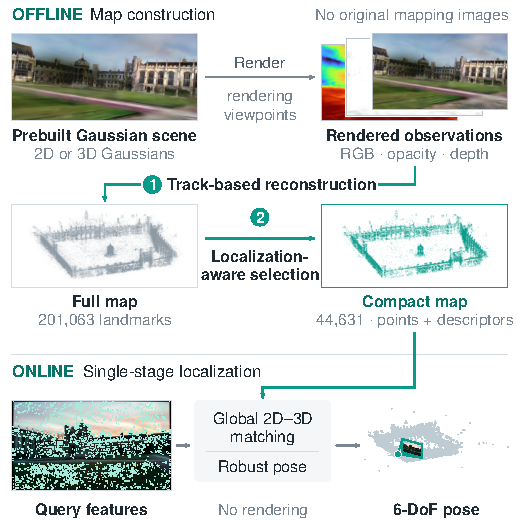
\includegraphics[width=\linewidth]{Fig2_overview.pdf}
\caption{Offline map construction and online localization. Rendered reference views provide observations for track reconstruction and compact-map selection. The deployed map stores coordinates and descriptors; a real query is localized by direct 2D--3D matching and robust pose estimation. Default map construction requires no original mapping images.}
\label{fig:fig2}
\end{figure}


Given a prebuilt Gaussian scene, AnyGSLoc constructs an explicit landmark map offline and then removes the renderer from the localization path. The construction follows the dependency of the information itself: rendered reference observations are first made reliable and associated into tracks; each track is then converted into a 3D landmark with a descriptor and uncertainty; finally, the candidate landmarks are selected according to their value for localization. Figure~\ref{fig:fig2} gives the complete pipeline. Thus, tracks provide the correspondence evidence, reconstruction turns that evidence into localization landmarks, and selection determines which landmarks need to be deployed.

\subsection{Problem Formulation and Map Representation}
\label{sec:overview}

Let a prebuilt Gaussian scene be $\mathcal G$. We choose reference cameras $\{(K_m,R_m,t_m)\}_{m=1}^{M}$ and render RGB $I_m$, opacity $\alpha_m$, and depth $Z_m$. Poses map world coordinates to camera coordinates, so the camera center is $C_m=-R_m^\mathsf Tt_m$ and the image projection is $\pi_m(X)=\operatorname{proj}(K_m(R_mX+t_m))$, where $\operatorname{proj}$ denotes perspective division. These cameras are rendering viewpoints and need not coincide with the original mapping cameras. The default pipeline uses rendered observations; the optional use of original mapping images is evaluated in Sec.~\ref{sec:input-availability}.

A localization landmark should represent one repeatedly observed image feature. Let $\mathcal T_i$ contain the observation indices $(m,k)$ belonging to landmark $i$, and let $\mathcal W_i$ be its supporting reference views. The reconstruction stage produces
\begin{equation}
\begin{aligned}
\mathcal A&=\{(X_i,d_i,\mathcal T_i,q_i,\Sigma_i^X)\}_{i=1}^{N},\\
\mathcal M_S&=\{(X_i,d_i):i\in S\},\qquad S\subseteq\{1,\ldots,N\}.
\end{aligned}
\label{eq:landmark}
\end{equation}
Here $X_i\in\mathbb R^3$ and the unit descriptor $d_i\in\mathbb R^{D_f}$ are the deployed landmark attributes. The scalar quality $q_i$ and approximate position covariance $\Sigma_i^X$ guide offline selection. We call $\mathcal A$ the \emph{Full} candidate bank and $\mathcal M_S$ the \emph{Compact} map. After export, localization needs only these landmark records and their search index; the Gaussian scene is no longer queried.

\subsection{Track Construction from Rendered Observations}
\label{sec:observations}
\label{sec:construction}
\begin{figure*}[t]
\centering
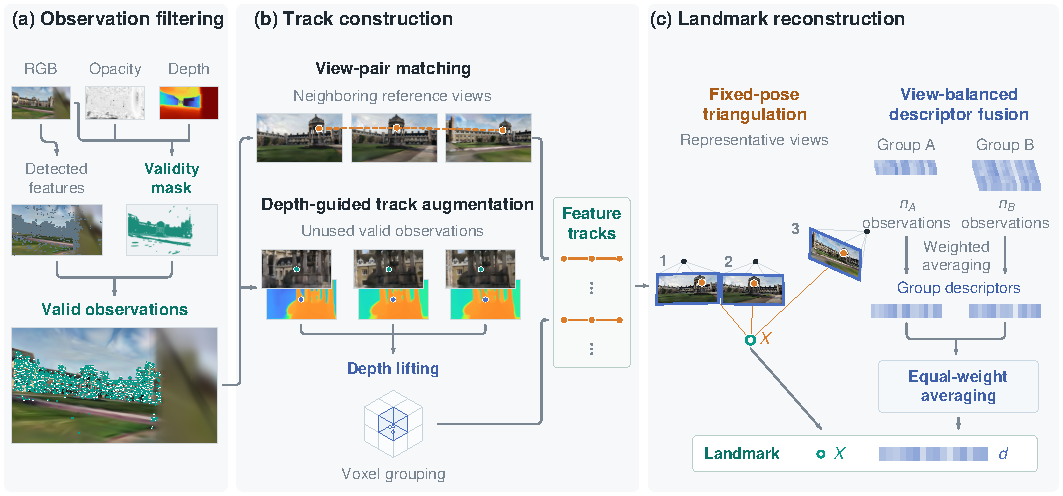
\includegraphics[width=\linewidth]{Fig3_reconstruction.pdf}
\caption{Rendering-aware landmark construction. (a) Observation filtering combines rendered RGB structure, opacity, and depth into a validity mask before cross-view association. (b) View-pair matching and depth-guided augmentation form geometrically verified tracks. (c) Fixed-pose triangulation estimates coordinates; view-balanced aggregation forms one descriptor per track. The example tracks use the MAtCha configuration evaluated in Table~\ref{tab:t8}.}
\label{fig:fig3}
\end{figure*}


The first stage determines which rendered detections should be treated as observations of the same scene feature. A strong detector response is not sufficient: rendering artifacts or weakly supported regions can yield distinctive but unreliable observations. We therefore filter detections before association and use calibrated epipolar geometry to verify the correspondences that form each track.

\paragraph{Observation filtering}
Frozen SuperPoint~\cite{detone2018superpoint} detects features on the complete rendered RGB image. For detection $o_{mk}=(u_{mk},d_{mk},s_{mk})$, $u_{mk}$ is the image coordinate, $d_{mk}$ is its unit descriptor, and $s_{mk}$ is its detector score. We evaluate three complementary validity tests at the detection location: geometric support $v_m^{\rm geom}$ from opacity and depth, local appearance support $v_m^{\rm app}$ from image structure, and region validity $v_m^{\rm reg}$ for unreliable image regions. Their conjunction defines the observations admitted to cross-view association:
\begin{equation}
\begin{aligned}
v_m(u)&=v_m^{\rm geom}(u)v_m^{\rm app}(u)v_m^{\rm reg}(u),\\
\mathcal O_m&=\{o_{mk}:v_m(u_{mk})=1\}.
\end{aligned}
\label{eq:observation_filter}
\end{equation}
The filter is applied after feature extraction and therefore controls the observations entering association rather than modifying the image seen by SuperPoint.

\paragraph{Geometrically verified tracks}
The retained observations are associated over a sparse graph of neighboring reference cameras. Descriptor similarity proposes candidate matches, while calibrated epipolar geometry rejects incompatible pairs; reciprocity and similarity margins further suppress ambiguous associations. Each accepted edge receives a confidence combining descriptor agreement, epipolar consistency, and detector support. The observation confidence $\gamma_{mi}$ is taken from the strongest accepted incident edge in the primary graph.

We merge accepted edges into tracks in confidence order, giving precedence to associations supported by three-view cycles over isolated chains. A merge is rejected if it would assign two detections from the same camera to one track. Consequently, each track contains at least three views and tracks have disjoint observation ownership. The notation $u_{mi}$, $d_{mi}$, and $s_{mi}$ is therefore unambiguous for $m\in\mathcal W_i$.

\paragraph{Depth-guided track augmentation}
The sparse camera graph does not necessarily connect every useful observation. For unmatched valid detections, rendered depth supplies a coarse world-space location that narrows the search for compatible associations. Candidate matches are then checked by descriptor similarity and epipolar consistency, producing additional tracks under the same one-observation-per-camera and disjoint-ownership constraints. Depth is used here to augment correspondence discovery, not to define the exported coordinate; both association paths feed the same track-based reconstruction in Fig.~\ref{fig:fig3}(b).

\subsection{Track-Based Landmark Reconstruction}
\label{sec:geometry}

A track supplies multiple image measurements of one scene feature. The reconstruction stage turns those measurements into the attributes required by the localization map: a 3D coordinate, a descriptor, and evidence for later selection. The key geometric choice is to let the matched pixels determine the coordinate. A Gaussian center is tied to a rendering primitive, whereas rendered depth provides a view-dependent distance estimate. Neither is guaranteed to be the point that best explains the feature correspondence. We therefore reconstruct the landmark from the calibrated rays associated with its track (Fig.~\ref{fig:fig3}(c)).

\paragraph{Robust multiview triangulation}
Let $\bar u_{mi}$ denote the homogeneous pixel-center coordinate of observation $u_{mi}$. Its unit world bearing is
$r_{mi}=\operatorname{normalize}(R_m^\mathsf TK_m^{-1}\bar u_{mi})$,
and $P_{mi}=I_3-r_{mi}r_{mi}^\mathsf T$ projects onto the plane orthogonal to that bearing. We retain a confidence-ranked geometry subset $\mathcal V_i\subseteq\mathcal W_i$ and estimate the point by minimizing its weighted ray distances:
\begin{equation}
X_i(w)=\arg\min_X\sum_{m\in\mathcal V_i}w_{mi}\lVert P_{mi}(X-C_m)\rVert^2.
\label{eq:triangulation}
\end{equation}
For fixed nonnegative weights, the solution satisfies
\begin{equation}
\begin{aligned}
A_i(w)X_i(w)&=b_i(w),\\
A_i(w)&=\sum_{m\in\mathcal V_i}w_{mi}P_{mi},\\
b_i(w)&=\sum_{m\in\mathcal V_i}w_{mi}P_{mi}C_m.
\end{aligned}
\label{eq:raynormal}
\end{equation}
Thus the coordinate is determined by the calibrated image observations. When the retained bearings are nondegenerate, the normal matrix is positive definite and the estimate is unique~\cite{hartley2004mvg}.

Associations can still contain individual outliers, so we refine the point by reweighting observations according to their reprojection residuals. Let $\bar\gamma_{mi}$ be the normalized base confidence, $z_{mi}^{(t)}$ the camera depth of the current estimate, and $e_{mi}^{(t)}=\lVert\pi_m(X_i^{(t)})-\bar u_{mi,1:2}\rVert_2$ the image residual. Starting from $X_i^{(0)}=X_i(w^{(0)})$ with $w_{mi}^{(0)}=\bar\gamma_{mi}$, each update is
\begin{equation}
\begin{aligned}
w_{mi}^{(t+1)}&=\bar\gamma_{mi}\,\mathbf 1[z_{mi}^{(t)}>0]\,
h_\delta(e_{mi}^{(t)}),\\
X_i^{(t+1)}&=X_i(w^{(t+1)}).
\end{aligned}
\label{eq:rayreweight}
\end{equation}
where $h_\delta(e)=\min\{1,\delta/\max(e,\epsilon)\}$ is a bounded decreasing residual weight. The cameras remain fixed throughout: only the observation weights change, and every update solves the same ray least-squares problem. The final finite, nondegenerate support set is denoted $\mathcal V_i^+$.

\paragraph{View-balanced descriptor fusion}
The track also provides the appearance evidence that will be stored with the reconstructed point. A flat average over all observations would implicitly weight a landmark by the sampling density of its reference views. We instead aggregate observations within pose groups and then give the occupied groups equal influence. For each group $\mathcal C_g$,
\begin{equation}
p_{ig}=\operatorname{normalize}\left(
\sum_{m\in\mathcal W_i\cap\mathcal C_g}a_{mi}d_{mi}
\right),
\label{eq:group_descriptor}
\end{equation}
where $a_{mi}$ combines detector and association confidence. We identify the group descriptor most representative of the others and retain a consistent subset of nearby group descriptors; let $\mathcal K_i$ denote their indices. The exported descriptor is
\begin{equation}
d_i=\operatorname{normalize}\left(
\sum_{g\in\mathcal K_i}p_{ig}
\right).
\label{eq:descriptor}
\end{equation}
This separates observation confidence from view-sampling density: confidence controls aggregation within a group, whereas equal group weights prevent repeated sampling of similar viewpoints from dominating the descriptor. Group-level trimming also limits inconsistent appearance, while deployment stores only one descriptor per landmark.

\paragraph{Quality and geometric uncertainty}
Selection needs two different kinds of evidence: whether a track is reliable and how strongly its position is constrained. Let $\bar e_i$ be the median reprojection residual over $\mathcal V_i^+$ and let $\theta_i$ denote a robust measure of track parallax. We define
\begin{equation}
\begin{aligned}
q_i&=\operatorname{clip}_{[0,1]}\left(q_i^{\rm geom}q_i^{\rm assoc}\right),\\
q_i^{\rm geom}&=\exp(-\bar e_i/\tau_e)
\min\left\{\theta_i/\tau_\theta,1\right\}.
\end{aligned}
\label{eq:landmark_quality}
\end{equation}
The association factor summarizes descriptor agreement and, for primary tracks, edge confidence, view-group support, and cycle evidence. Its exact aggregation and fallback rules are implementation details in Sec.~\ref{sec:implementation}; descriptor agreement used for quality is computed from the track mean independently of the exported group-balanced descriptor.

A scalar score does not reveal directional uncertainty. For example, a narrow-baseline track can have a small reprojection residual while remaining weakly constrained along depth. Let $J_{X,mi}=\left.\partial\pi_m(X)/\partial X\right|_{X_i}$ be the $2\times3$ point-projection Jacobian. Conditional on fixed cameras and associations, we approximate
\begin{equation}
\Sigma_i^X=\widehat\sigma_i^2
\left(\sum_{m\in\mathcal V_i^+}\widehat w_{mi}
J_{X,mi}^{\mathsf T}J_{X,mi}\right)^{-1},
\label{eq:pointcov}
\end{equation}
where $\widehat w_{mi}$ are evaluated at the final estimate and $\widehat\sigma_i^2$ is a robust residual scale. This covariance captures the anisotropy of the reconstructed point and is later propagated into the pose-information model.

\subsection{Localization-Aware Landmark Selection}
\label{sec:selection}
\begin{figure*}[t]
\centering
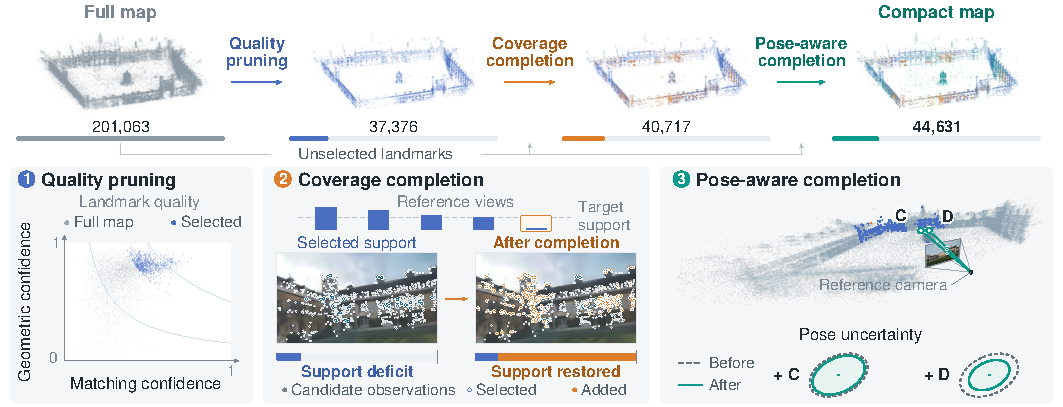
\includegraphics[width=\linewidth]{Fig4_selection.pdf}
\caption{Localization-aware selection on the Great Court 3DGS map. Quality pruning and coverage completion retain 37,376 and 40,717 points. Pose completion adds 4,096 points and cleanup removes 182, leaving 44,631. The lower panels illustrate quality, coverage, and complementary pose constraints; contour changes are emphasized for visibility.}
\label{fig:fig4}
\end{figure*}


The candidate bank is richer than the map that needs to be deployed. Selection therefore asks a different question from reconstruction: not whether a landmark is valid, but whether retaining it adds useful localization support. A quality-only ranking favors strong individual points but can leave some reference views weakly supported; coverage alone can fill those views with redundant points. We therefore proceed in three stages: establish a reliable quality core, restore deficient reference-view support, and add landmarks that contribute complementary local pose information. The final stage also removes coverage-only landmarks that have become redundant. Figure~\ref{fig:fig4} and Algorithm~\ref{alg:selection} summarize the process.

\paragraph{Quality pruning and coverage completion}
For a selected set $S$, define the support of reference view $m$ and the coverage objective by
\begin{equation}
\begin{aligned}
r_m(S)&=\sum_{i\in S}\mathbf 1[m\in\mathcal W_i],\\
b_m&=\min\{b,r_m(\{1,\ldots,N\})\},\\
F_{\rm cov}(S)&=\sum_{m=1}^{M}\omega_m\min\{r_m(S),b_m\}.
\end{aligned}
\label{eq:matchobjective}
\end{equation}
Because observation ownership is disjoint, $r_m(S)$ counts distinct selected features in view $m$. The target $b_m$ prevents the selector from demanding support unavailable in the Full bank, while $\omega_m$ balances reference-camera groups.

Quality pruning initializes $S$ with a quality-ranked prefix until the core support criterion is met. Coverage completion then adds the candidate with the largest marginal increase in $F_{\rm cov}$, directing additions toward views that remain below their targets. These coverage additions are recorded because some may become redundant after pose-aware completion.

\paragraph{Pose-aware completion}
Once basic coverage is available, candidates should be judged by the pose constraints they add to the current map. We linearize projection at each reference camera using a left pose perturbation $\delta\xi=(\delta t^\mathsf T,\delta\theta^\mathsf T)^\mathsf T$. Let $J_{\xi,mi}$ be the corresponding $2\times6$ projection Jacobian and define $\widetilde J_{mi}=J_{\xi,mi}D$, where $D=\operatorname{diag}(s_tI_3,s_rI_3)$ fixes the relative translation and rotation scales. The point Jacobian above propagates landmark uncertainty into the image plane:
\begin{equation}
\begin{aligned}
\Sigma^u_{mi}&=\sigma_{\rm pix}^2I_2+
J_{X,mi}\Sigma_i^XJ_{X,mi}^{\mathsf T},\\
B_{mi}&=q_{mi}\widetilde J_{mi}^{\mathsf T}
(\Sigma^u_{mi})^{-1}\widetilde J_{mi},\\
H_m(S)&=\lambda I_6+
\sum_{i\in S:\,m\in\mathcal W_i}B_{mi}.
\end{aligned}
\label{eq:information}
\end{equation}
The weight $q_{mi}$ combines landmark quality with observation support, while the covariance term attenuates uncertain landmark locations. Candidate contributions $B_{mi}$ are computed before selection; $H_m(S)$ records the information supplied by the landmarks already retained.

We rank an unselected landmark by its conditional information gain:
\begin{equation}
G_i(S)=\sum_{m\in\mathcal W_i}\left[
\log\frac{\det(H_m(S)+B_{mi})}{\det H_m(S)}
+\beta h_{mi}(S)
\right].
\label{eq:posegain}
\end{equation}
The log-determinant term measures the reduction in local pose-uncertainty volume and therefore favors constraints in directions that remain weakly observed. The diversity term $h_{mi}(S)$ rewards categories not yet represented by the selected map. After each accepted landmark, the information matrices and occupied categories are updated, so each candidate is evaluated relative to the map already built.

Pose completion also absorbs the final redundancy cleanup. We revisit only the landmarks introduced during coverage completion and remove one when its affected views still meet the support level attained at the start of cleanup. The targets remain fixed during deletion, so pose-added landmarks can replace redundant coverage-only points without altering the quality core or pose additions. Selection changes only which rows of $\mathcal A$ are retained; the reconstructed coordinates and descriptors are never modified.

\par\medskip
\noindent\begin{minipage}{\linewidth}
\refstepcounter{anygsalgorithm}\label{alg:selection}
\hrule\smallskip
\textbf{Algorithm \theanygsalgorithm. Localization-aware landmark selection}
\smallskip\hrule\smallskip
\small
\textbf{Input:} Candidate bank $\mathcal A$, target support $b$, and selection settings.\\[2pt]
\textbf{1. Quality pruning.} Retain a quality-ranked prefix in $S$ until the core stopping criterion is met.\\[2pt]
\textbf{2. Coverage completion.} While feasible deficits remain, add the candidate with largest positive marginal gain in $F_{\rm cov}$. Record these additions as $\mathcal U_{\rm cov}$.\\[2pt]
\textbf{3. Pose-aware completion.} Add admissible candidates using refreshed $G_i(S)$, updating the information matrices and occupied categories until a stopping criterion is met.\\[2pt]
\hspace*{1em}\emph{Final cleanup:} Freeze $\tau_m=\min\{b,r_m(S)\}$. Visit $\mathcal U_{\rm cov}$ in increasing quality; remove a point only if all affected views retain $\tau_m$.\\[2pt]
\textbf{Output:} $\mathcal M_S=\{(X_i,d_i):i\in S\}$.
\smallskip\hrule
\end{minipage}
\par\medskip


\subsection{Single-Stage Query Localization}
\label{sec:localization}

The exported map is directly compatible with a structure-based localizer. We extract query features with the same frozen SuperPoint encoder, match each query descriptor to the highest-similarity landmark descriptor, and pass the retained correspondences to a single PoseLib call with robust estimation and local optimization~\cite{poselib,fischler1981ransac}. Matching and solver details are fixed in Sec.~\ref{sec:implementation}. No image retrieval, Gaussian rendering, or separate dense refinement is required online.

For $K$ query descriptors, exhaustive descriptor search requires $O(K|S|D_f)$ arithmetic, while the stored coordinate--descriptor arrays contain $(3+D_f)|S|$ values. Map selection therefore reduces both the persistent landmark representation and the number of descriptor comparisons while preserving the same online localization procedure.
\section{Experiments}
\label{sec:experiments}

We evaluate AnyGSLoc from four complementary perspectives. First, we compare the resulting localization map with established methods on standard benchmarks. Second, we isolate the geometric and appearance decisions used to construct a landmark. Third, we examine whether localization-aware selection can reduce the deployed map without sacrificing the useful part of its localization accuracy. Finally, we test the construction pipeline across different Gaussian representations and with optional access to the original mapping images.

\subsection{Experimental Setup}
\label{sec:setup}

\paragraph{Data and map variants}
We use Cambridge Landmarks, 7Scenes, and 12Scenes~\cite{kendall2015posenet,shotton2013scenes,valentin2016energy}, comprising five outdoor and nineteen indoor scenes with 24,700 queries. Cambridge uses vanilla 3DGS by default, while the indoor experiments use 2DGS and SfM pseudo-ground-truth poses~\cite{brachmann2021pgt}. All local comparisons and ablations use the same 1,918 Cambridge queries. Unless stated otherwise, AnyGSLoc results use \emph{Compact}, the final selected map. \emph{Full} denotes the complete candidate bank before selection and provides the reference for measuring the effect of map compression. Selection does not modify a retained landmark's coordinate or descriptor.

\paragraph{Metrics and comparisons}
Translation error (TE) is the camera-center distance and rotation error (RE) is the relative rotation angle. For each scene, we compute the requested statistic over its queries and then average the scene-level values with equal weight. This convention is used for medians, means, percentiles, and recall, so a scene with many queries does not dominate the aggregate. R5 and R15 denote the fractions within $5$\,cm/$5^\circ$ and $15$\,cm/$5^\circ$, respectively. All returned estimates, including severe failures, remain in the statistics. Landmark counts and storage are summed over scenes, with MB denoting $10^6$ bytes. Tables~\ref{tab:t1}--\ref{tab:t3} reproduce published results at their reported precision and scene coverage; they are therefore literature comparisons rather than identical-input reruns.

\paragraph{Localization time and storage}
All local timing measurements use an RTX~3090 and four CPU threads, with three fresh processes per scene, 50 warm-up queries, and the same 100 measured queries per process. We report a single metric, \emph{localization time}, from fresh query feature extraction through the final pose output. Decoding, initialization, external preprocessing, and segmentation-network inference are outside this boundary. Native solver and diagnostic operations are retained for each baseline. Means are scene-equal. Storage counts scene-specific deployment assets while excluding shared pretrained weights, query inputs, and training intermediates. These definitions are kept fixed across the local comparison and ablation experiments.

\subsubsection{Implementation settings}
\label{sec:implementation}
We use the same construction rules across the evaluated Gaussian representations. This subsection collects numerical settings and exact aggregation rules; the preceding method section describes their roles. Reference images are rendered at the original mapping poses and intrinsics in all reported experiments.

\paragraph{Observation filtering}
Mask values are sampled at rounded detector coordinates after feature extraction. Geometric support requires finite positive depth, finite opacity at least 0.05, and a maximum horizontal/vertical backward depth difference no larger than 8\% of the median positive image depth. Appearance support is the larger of the normalized local Sobel magnitude and intensity variation, thresholded at 0.20. Each component is divided by its 0.97 quantile and clipped to $[0,1]$. The averaging window and mask-dilation radius scale from 9 and 5 pixels at a 1080-pixel short side; the averaging window is odd and at least three pixels. Region validity excludes a border of $\max\{1,\operatorname{round}(0.02\min(H,W))\}$ pixels. Available distortion is invalid when nonfinite or when its absolute value exceeds both its median plus 20 median absolute deviations and its 0.995 quantile; the deviation floor is $10^{-8}$. Missing distortion adds no rejection criterion.

\paragraph{Track association}
The camera graph unions up to six neighbors per view. Eligible pairs have a baseline of 0.03--5\,m and an optical-axis angle no larger than $75^\circ$; pairs are ranked by normalized baseline plus $0.5(1-\cos\theta)$. Normalization uses the median eligible baseline. Matching tests the four leading descriptor candidates in each direction, with a 2-pixel symmetric epipolar threshold, cosine similarity at least 0.65, and two-sided margin 0.01. A missing valid runner-up has score $-\infty$. For a pair in views $a,b$, the accepted-edge confidence is
$\gamma_{ab}=\langle d_a,d_b\rangle\exp[-e_{ab}^2/(2\sigma_e^2)]\sqrt{s_as_b}$,
with $\sigma_e=2$\,px. Depth-guided augmentation uses up to 256 strongest unused valid observations per view, 0.05-m world voxels, similarity 0.70, margin 0.01, and the same epipolar test. Augmented tracks require three cameras spanning at least two pose groups.

\paragraph{Triangulation and descriptor fusion}
Detector coordinates are converted to physical pixel centers using $\bar u=(u_x+0.5,u_y+0.5,1)^\mathsf T$. Geometry uses the 32 highest-confidence observations per track. Base confidence is floored at $10^{-4}$ and divided by its within-track mean. After the initial ray solve, three reweighting updates use $\delta=2$\,px. Ray and final pixel-Jacobian normal matrices must have finite spectra and minimum eigenvalues above $10^{-12}$; at least three finite, positive-depth observations are required. The variance scale in~\eqref{eq:pointcov} is
$\widehat\sigma_i^2=\max\{\operatorname{median}_{m\in\mathcal V_i^+}e_{mi}^2,10^{-8}\,\mathrm{px}^2\}$.

Camera groups are formed by deterministic farthest-point grouping in an embedding of median-centered, scale-normalized camera centers and optical axes weighted by 0.5. The positional scale is the median positive distance from the median camera center. The first group representative is farthest from the embedding centroid; later representatives maximize distance to the current set, and cameras are assigned to their nearest representative. We use at most eight groups. Fusion weights are $a_{mi}=\max\{s_{mi}\gamma_{mi},10^{-4}\}$. For $n_i^{\rm grp}$ occupied groups, $\mathcal K_i$ contains the $\max\{1,\operatorname{round}(0.8n_i^{\rm grp})\}$ descriptors nearest to the cosine medoid. Stored descriptors have $D_f=256$ dimensions.

\paragraph{Landmark quality}
The geometric scales are $\tau_e=2$\,px and $\tau_\theta=1^\circ$. Parallax $\theta_i$ is the 75th percentile of pairwise bearing angles among positive-depth support observations with residual at most 4\,px. If fewer than three satisfy this residual threshold, all finite positive-depth support observations are used instead.

For association reliability, let $\bar\gamma_i$ be the mean observation confidence, $c_i$ the mean cosine agreement with the normalized unweighted track-mean descriptor (clipped to $[0,1]$), and $g_i=\min\{n_i^{\rm grp}/3,1\}$. Then
\begin{equation}
q_i^{\rm assoc}=\begin{cases}
\chi_i(\bar\gamma_i c_i g_i)^{1/3},&\text{primary track},\\
c_i,&\text{augmented track},
\end{cases}
\label{eq:quality_implementation}
\end{equation}
where $\chi_i=1$ for cycle-seeded tracks and $0.8$ for pure chains. Each factor in the primary-track product is floored at $10^{-8}$ for numerical stability, and the final quality is clipped to $[0,1]$. The track mean used here is distinct from the exported descriptor in~\eqref{eq:descriptor}.

\paragraph{Selection settings}
Quality ranking resolves ties by decreasing track length and then candidate ID. The core contains at least 1,024 points and checks the tenth percentile of per-view support every 512 additions, against target $b=256$; candidate exhaustion terminates the step. Coverage completion clips each target to Full-map feasibility, balances groups with $\omega_m=\sqrt{\bar n/n_{g(m)}}$ for group size $n_g$ and mean size $\bar n$, and resolves equal marginal gains by quality then ID.

For the evaluated pinhole cameras, let $y_{mi}=R_mX_i+t_m$. The left-increment pose Jacobian used in~\eqref{eq:information} is
$J_{\xi,mi}=J_{X,mi}R_m^\mathsf T[I_3\;- [y_{mi}]_\times]$,
using the previously defined point Jacobian. Task scales are $s_t=0.05$\,m and $s_r=5\pi/180$ radians, with $\sigma_{\rm pix}^2=4$\,px$^2$, $\lambda=10^{-4}$, and $\beta=0.05$. Computation uses the pseudoinverse of $\Sigma^u_{mi}+10^{-8}I_2$ and symmetrizes $B_{mi}$. A nonfinite stored point covariance is omitted from image-noise propagation.

The detector-conditioned weight is
\begin{equation}
q_{mi}=q_i\left[\frac12+\frac12\operatorname{clip}_{[0,1]}
\left(\frac{s_{mi}-s_{m,10}}{\max\{s_{m,90}-s_{m,10},10^{-6}\}}\right)\right],
\label{eq:detector_weight_implementation}
\end{equation}
where $s_{m,10}$ and $s_{m,90}$ are per-view detector-score percentiles. The bracketed factor is one if fewer than two finite scores are available. All candidate-view information contributions remain fixed during selection.

Diversity counts previously unoccupied categories using a $4\times4$ image grid, depth index $\lfloor2\log_2\max(z_{mi},0.05)\rfloor$ with depth in meters, and 0.5-m world voxels. Pose completion accepts at most 4,096 landmarks and three additions per voxel. Scores are refreshed before acceptance, and the process stops below 2\% of its first accepted gain, at nonpositive gain, or on exhaustion. Voxel limits apply only to pose additions. Cleanup targets are frozen at the distinct support attained before cleanup, capped at $b$; only coverage-added landmarks can be removed.

\paragraph{Query settings}
Exact float32 descriptor matching uses chunks of 8,192 map rows; equal similarities select the smaller map row. Given $K$ matches, we retain $\min\{K,\max(256,\lceil0.65K\rceil)\}$ by score, without reciprocal filtering or duplicate-landmark removal. Fewer than four correspondences return failure. PoseLib uses confidence 0.999 and 250--30,000 RANSAC iterations. The query feature budget is $\operatorname{clip}_{[1024,2048]}(\operatorname{round}(2048A_{\rm med}/2073600))$, and the reprojection threshold is $\max\{2,0.007176913f_{\rm med}\}$\,px. Here $A_{\rm med}$ is the median reference-image area and $f_{\rm med}$ the median geometric mean of its horizontal and vertical focal lengths. Localization-time boundaries remain those defined in Sec.~\ref{sec:setup}.


\subsection{Benchmark Localization Accuracy}
\label{sec:accuracy}
\begin{table}[!t]
\centering
\fontsize{7.1}{8.5}\selectfont
\setlength{\tabcolsep}{1.0pt}
\renewcommand{\arraystretch}{1.03}
\caption{Localization on Cambridge Landmarks}\label{tab:t1}
\begin{tabular}{@{}lcccccc@{}}
\toprule
Method & Court & College & Hospital & Shop & Church & Mean \\
\midrule
\multicolumn{7}{@{}l}{\textit{Feature matching}} \\
AS (SIFT)~\cite{reported260504730v1bibbib55} & 24/0.13 & 13/0.22 & 20/0.36 & 4/0.21 & 8/0.25 & 14/0.23 \\
HLoc (SP+SG)~\cite{sarlin2019hloc} & 17.7/0.11 & \textbf{11.0}/0.20 & 15.1/0.31 & 4.2/0.20 & 7.0/0.22 & 11.0/0.21 \\
PixLoc~\cite{reported260504730v1bibbib20} & 30/0.1 & 14/0.2 & 16/0.3 & 5/0.2 & 10/0.3 & 15/0.2 \\
\midrule
\multicolumn{7}{@{}l}{\textit{Pose regression}} \\
DFNet~\cite{reported260504730v1bibbib26} & -- & 73/2.37 & 200/2.98 & 67/2.21 & 137/4.02 & 119/2.90 $^\dagger$ \\
LENS~\cite{reported260504730v1bibbib29} & -- & 33/0.5 & 44/0.9 & 27/1.6 & 53/1.6 & 39/1.2 $^\dagger$ \\
PMNet~\cite{reported260504730v1bibbib28} & -- & 31/0.55 & 44/0.79 & 17/0.86 & 31/0.96 & 31/0.79 $^\dagger$ \\
\midrule
\multicolumn{7}{@{}l}{\textit{Scene-coordinate regression}} \\
DSAC*~\cite{brachmann2021dsacstar} & 33.0/0.21 & 17.9/0.31 & 21.1/0.40 & 5.2/0.24 & 15.4/0.51 & 18.5/0.33 \\
ACE (Poker)~\cite{brachmann2023ace} & 28/0.1 & 18/0.3 & 25/0.5 & 5/0.3 & 9/0.3 & 17/0.3 \\
NeuMap~\cite{reported260504730v1bibbib7} & \textbf{6}/0.10 & 14/0.19 & 19/0.36 & 6/0.25 & 17/0.53 & 12/0.29 \\
GLACE~\cite{reported260504730v1bibbib37} & 19/0.1 & 19/0.3 & 17/0.4 & 4/0.2 & 9/0.3 & 14/0.3 \\
\midrule
\multicolumn{7}{@{}l}{\textit{NeRF / Gaussian scene methods}} \\
CROSSFIRE~\cite{reported260504730v1bibbib42} & -- & 47/0.7 & 43/0.7 & 20/1.2 & 39/1.4 & 37/1.0 $^\dagger$ \\
DFNet+NeFeS50~\cite{reported260504730v1bibbib27} & -- & 37/0.54 & 52/0.88 & 15/0.53 & 37/1.14 & 35/0.77 $^\dagger$ \\
HR-APR~\cite{reported260504730v1bibbib58} & -- & 36/0.58 & 53/0.89 & 13/0.51 & 38/1.16 & 35/0.78 $^\dagger$ \\
NeRFMatch~\cite{zhou2024nerfmatch} & 19.6/0.09 & \underline{12.5}/0.23 & 20.9/0.38 & 8.4/0.40 & 10.9/0.35 & 14.5/0.29 \\
MCLoc~\cite{reported260504730v1bibbib57} & -- & 31/0.42 & 39/0.73 & 12/0.45 & 26/0.88 & 27/0.62 $^\dagger$ \\
GSplatLoc~\cite{reported260504730v1bibbib47} & -- & 31/0.49 & 16/0.68 & 4/0.34 & 14/0.42 & 16/0.48 $^\dagger$ \\
GSFFs-PR Feature~\cite{reported260504730v1bibbib52} & -- & 17/0.26 & 18/0.36 & 4/0.25 & 8/0.26 & 12/0.30 $^\dagger$ \\
STDLoc~\cite{huang2025stdloc} & 15.7/0.06 & 15.0/\underline{0.17} & 11.9/0.21 & 3.0/0.13 & 4.7/0.14 & 10.1/0.14 \\
ACE+GS-CPR~\cite{reported260504730v1bibbib61} & -- & 20/0.29 & 21/0.40 & 5/0.24 & 13/0.40 & 15/0.33 $^\dagger$ \\
ULF-Loc~\cite{gu2026ulfloc} & \underline{7.49}/\textbf{0.04} & 17.03/0.19 & \underline{10.26}/\underline{0.19} & 2.83/0.14 & 3.65/\textbf{0.11} & \underline{8.3}/\underline{0.13} \\
PNeRFLoc~\cite{reported250319358v1bibbib68} & 81/0.25 & 24/0.29 & 28/0.37 & 6/0.27 & 40/0.55 & 35.8/0.35 \\
SplitGS-Loc~\cite{lee2026splitgsloc} & 9.3/0.06 & 14.1/\underline{0.17} & 13.8/0.29 & 2.5/0.12 & 3.8/\underline{0.13} & 8.7/0.15 \\
GSVisLoc~\cite{khatib2025gsvisloc} & -- & 23/0.3 & 22/0.42 & 8/0.29 & 14/0.45 & 17/0.36 $^\dagger$ \\
\midrule
AnyGSLoc (Full) & 8.12/\textbf{0.04} & 16.48/\underline{0.17} & \textbf{9.26}/\textbf{0.17} & \underline{2.07}/\underline{0.10} & \textbf{3.16}/\textbf{0.11} & \textbf{7.82}/\textbf{0.12} \\
AnyGSLoc (Compact) & 9.33/\underline{0.05} & 17.40/\textbf{0.16} & 10.57/\underline{0.19} & \textbf{2.02}/\textbf{0.09} & \underline{3.37}/\textbf{0.11} & 8.54/\textbf{0.12} \\
\bottomrule
\end{tabular}
\tabnote{Median TE/RE in cm/degrees. Means average scene medians. Compact is our final map; Full retains all candidate landmarks. $\dagger$: four-scene result without Great Court, excluded from aggregate highlighting. Literature values follow the cited sources; bold and underlining mark best and second-best values at reported precision.}
\end{table}

\begin{table*}[!t]
\centering
\footnotesize
\setlength{\tabcolsep}{1.5pt}
\renewcommand{\arraystretch}{1.10}
\caption{Localization on 7Scenes}\label{tab:t2}
\begin{tabular*}{\linewidth}{@{\extracolsep{\fill}}lcccccccc@{}}
\toprule
Method & Chess & Fire & Heads & Office & Pumpkin & Kitchen & Stairs & Mean \\
\midrule
\multicolumn{9}{@{}l}{\textit{Feature matching}} \\
AS (SIFT)~\cite{reported260504730v1bibbib55} & 3/0.87 & 2/1.01 & 1/0.82 & 4/1.15 & 7/1.69 & 5/1.72 & 4/1.01 & 3.71/1.18 \\
HLoc (SP+SG)~\cite{sarlin2019hloc} & 2.39/0.84 & 2.29/0.91 & 1.13/0.77 & 3.14/0.92 & 4.92/1.30 & 4.22/1.39 & 5.05/1.41 & 3.31/1.08 \\
DVLAD+R2D2~\cite{reported260504730v1bibbib56} & 2.56/0.88 & 2.21/0.86 & 0.98/0.75 & 3.48/1.00 & 4.79/1.28 & 4.21/1.44 & 4.60/1.27 & 3.26/1.07 \\
\midrule
\multicolumn{9}{@{}l}{\textit{Pose regression}} \\
DFNet~\cite{reported260504730v1bibbib26} & 3/1.12 & 6/2.30 & 4/2.29 & 6/1.54 & 7/1.92 & 7/1.74 & 12/2.63 & 6/1.93 \\
PMNet~\cite{reported260504730v1bibbib28} & 3/1.26 & 4/1.76 & 2/1.68 & 6/1.69 & 7/1.96 & 8/2.23 & 11/2.97 & 6/1.93 \\
Marepo~\cite{reported260504730v1bibbib24} & 1.9/0.83 & 2.3/0.92 & 2.1/1.24 & 2.9/0.93 & 2.5/0.88 & 2.9/0.98 & 5.9/1.48 & 2.9/1.04 \\
\midrule
\multicolumn{9}{@{}l}{\textit{Scene-coordinate regression}} \\
DSAC*~\cite{brachmann2021dsacstar} & 0.50/0.17 & 0.78/0.29 & 0.50/0.34 & 1.19/0.35 & 1.19/0.29 & 0.72/0.21 & 2.65/0.78 & 1.07/0.35 \\
ACE~\cite{brachmann2023ace} & 0.55/0.18 & 0.83/0.33 & 0.53/0.33 & 1.05/0.29 & 1.06/0.22 & 0.77/0.21 & 2.89/0.81 & 1.10/0.34 \\
NeuMap~\cite{reported260504730v1bibbib7} & 2/0.81 & 3/1.11 & 2/1.17 & 3/0.98 & 4/1.11 & 4/1.33 & 4/1.12 & 3.14/0.95 \\
GLACE~\cite{reported260504730v1bibbib37} & 0.6/0.18 & 0.9/0.34 & 0.6/0.34 & 1.1/0.29 & 0.9/0.23 & 0.8/0.20 & 3.2/0.93 & 1.2/0.36 \\
NBE+SLD~\cite{reported250319358v1bibbib15} & 0.6/0.18 & 0.7/0.26 & 0.6/0.35 & 1.3/0.33 & 1.5/0.33 & 0.8/0.19 & 2.6/0.72 & 1.16/0.34 \\
\midrule
\multicolumn{9}{@{}l}{\textit{NeRF / Gaussian scene methods}} \\
DFNet+NeFeS50~\cite{reported260504730v1bibbib27} & 2/0.57 & 2/0.74 & 2/1.28 & 2/0.56 & 2/0.55 & 2/0.57 & 5/1.28 & 2.4/0.79 \\
HR-APR~\cite{reported260504730v1bibbib58} & 2/0.55 & 2/0.75 & 2/1.45 & 2/0.64 & 2/0.62 & 2/0.67 & 5/1.30 & 2.4/0.85 \\
PNeRFLoc~\cite{reported250319358v1bibbib68} & 2/0.80 & 2/0.88 & 1/0.83 & 3/1.05 & 6/1.51 & 5/1.54 & 32/5.73 & 7.29/1.76 \\
NeRFMatch~\cite{zhou2024nerfmatch} & 0.95/0.30 & 1.11/0.41 & 1.34/0.92 & 3.09/0.87 & 2.21/0.60 & 1.03/0.28 & 9.26/1.74 & 2.71/0.73 \\
MCLoc~\cite{reported260504730v1bibbib57} & 2/0.8 & 3/1.4 & 3/1.3 & 4/1.3 & 5/1.6 & 6/1.6 & 6/2.0 & 4.1/1.43 \\
GSplatLoc~\cite{reported260504730v1bibbib47} & 0.39/0.13 & 0.91/0.29 & 0.94/0.50 & 1.41/0.32 & 1.41/0.26 & 1.32/0.29 & 3.44/0.82 & 1.40/0.37 \\
GSFFs-PR Feature~\cite{reported260504730v1bibbib52} & 0.4/0.19 & 0.6/0.26 & 0.5/0.36 & 1.0/0.31 & 1.3/0.38 & 0.6/0.23 & 25.1/0.63 & 4.2/0.34 \\
STDLoc~\cite{huang2025stdloc} & 0.46/0.15 & 0.57/0.24 & 0.45/0.26 & 0.86/0.24 & 0.93/0.21 & 0.63/0.19 & 1.42/0.41 & 0.76/0.24 \\
ACE+GS-CPR~\cite{reported260504730v1bibbib61} & 0.5/0.15 & 0.6/0.25 & 0.4/0.28 & 0.9/0.26 & 1.0/0.23 & 0.7/0.17 & 1.4/0.42 & 0.8/0.25 \\
ULF-Loc~\cite{gu2026ulfloc} & 0.42/\underline{0.11} & \underline{0.44}/\underline{0.19} & \underline{0.36}/\textbf{0.21} & 0.73/0.20 & 0.92/\underline{0.18} & 0.65/0.13 & \underline{1.38}/\underline{0.36} & 0.7/\underline{0.20} \\
CROSSFIRE~\cite{reported260504730v1bibbib42} & 1/0.4 & 5/1.9 & 3/2.3 & 5/1.6 & 3/0.8 & 2/0.8 & 12/1.9 & 4.43/1.38 \\
SplitGS-Loc~\cite{lee2026splitgsloc} & 0.7/0.16 & 0.7/0.29 & 0.6/0.26 & 1.2/0.25 & 1.4/0.25 & 1.0/0.18 & 1.6/0.47 & 1.0/0.26 \\
SplitGS-Loc + GS-CPR~\cite{lee2026splitgsloc} & \underline{0.3}/\underline{0.11} & \textbf{0.4}/\textbf{0.18} & 0.4/0.27 & \textbf{0.6}/\textbf{0.16} & 0.9/0.20 & \textbf{0.4}/\underline{0.12} & \textbf{0.9}/\textbf{0.28} & \textbf{0.6}/\textbf{0.19} \\
GSVisLoc~\cite{khatib2025gsvisloc} & 0.39/0.13 & 0.58/0.24 & 0.54/0.34 & 1.0/0.26 & 0.90/0.21 & 0.73/0.18 & 4.7/0.96 & 1.3/0.33 \\
\midrule
AnyGSLoc (Full) & 0.32/\underline{0.11} & 0.57/0.24 & 0.42/0.25 & \underline{0.65}/0.19 & \underline{0.75}/\underline{0.18} & 0.44/\underline{0.12} & 1.95/0.58 & 0.73/0.24 \\
AnyGSLoc (Compact) & \textbf{0.27}/\textbf{0.09} & 0.53/0.22 & \textbf{0.35}/\underline{0.22} & \textbf{0.60}/\underline{0.17} & \textbf{0.69}/\textbf{0.17} & \underline{0.41}/\textbf{0.11} & 1.61/0.48 & \underline{0.64}/0.21 \\
\bottomrule
\end{tabular*}
\tabnote{Median TE/RE in cm/degrees; our results use SfM pseudo-ground-truth poses. Published values retain their original protocols and precision. SplitGS-Loc + GS-CPR adds pose refinement. Bold and underlining mark best and second-best values at reported precision.}
\end{table*}

\begin{table}[!t]
\centering
\footnotesize
\setlength{\tabcolsep}{2pt}
\renewcommand{\arraystretch}{1.15}
\caption{Localization on 12Scenes}\label{tab:t3}
\begin{tabular*}{\linewidth}{@{\extracolsep{\fill}}lccc@{}}
\toprule
Method & Apartments & Offices & All \\
\midrule
\multicolumn{4}{@{}l}{\textit{Pose regression}} \\
Marepo~\cite{reported260504730v1bibbib24} & 1.97/1.07 & 2.13/1.00 & 2.1/1.04 \\
\midrule
\multicolumn{4}{@{}l}{\textit{Scene-coordinate regression}} \\
SCRNet~\cite{reported260504730v1bibbib38} & 3.12/1.30 & 2.92/1.13 & 3.0/1.22 \\
SCRNet-ID~\cite{reported260504730v1bibbib62} & 2.52/1.07 & 3.02/1.17 & 2.8/1.12 \\
DSAC*~\cite{brachmann2021dsacstar} & -- & -- & 0.5/0.25 \\
ACE~\cite{brachmann2023ace} & 0.60/0.24 & 0.80/0.27 & 0.7/0.26 \\
GLACE~\cite{reported260504730v1bibbib37} & 0.57/0.25 & 0.72/0.26 & 0.7/0.25 \\
NeRF-SCR~\cite{reported260504730v1bibbib8} & 1.73/0.68 & 2.20/0.83 & 2.0/0.76 \\
\midrule
\multicolumn{4}{@{}l}{\textit{NeRF / Gaussian scene methods}} \\
PNeRFLoc~\cite{reported250319358v1bibbib68} & 2.33/0.97 & 3.30/1.22$^{\dagger}$ & 2.8/1.08$^{\dagger}$ \\
SplatLoc~\cite{zhai2025splatloc} & 1.13/0.48 & 1.32/0.52 & 1.2/0.50 \\
GSplatLoc~\cite{reported260504730v1bibbib47} & 1.08/0.24 & 1.64/0.28 & 1.4/0.26 \\
GSFFs-PR Feature~\cite{reported260504730v1bibbib52} & 0.45/0.24 & 0.72/0.31 & 0.6/0.27 \\
Marepo+GS-CPR~\cite{reported260504730v1bibbib61} & 0.59/0.28 & 0.72/0.26 & 0.7/0.28 \\
ACE+GS-CPR~\cite{reported260504730v1bibbib61} & 0.48/0.21 & 0.60/0.22 & 0.5/0.21 \\
STDLoc~\cite{huang2025stdloc} & 0.34/0.17 & 0.45/0.18 & 0.4/0.18 \\
ULF-Loc~\cite{gu2026ulfloc} & 0.30/\underline{0.15} & \underline{0.38}/\underline{0.16} & \underline{0.3}/0.15 \\
\midrule
AnyGSLoc (Full) & \textbf{0.20}/\textbf{0.10} & \textbf{0.31}/\textbf{0.13} & \textbf{0.26}/\underline{0.12} \\
AnyGSLoc (Compact) & \underline{0.21}/\textbf{0.10} & \textbf{0.31}/\textbf{0.13} & \textbf{0.26}/\textbf{0.11} \\
\bottomrule
\end{tabular*}
\tabnote{TE/RE in cm/degrees. Group columns average published scene medians (six scenes each); All retains published aggregates. Our values use unrounded scene medians and SfM pseudo-ground truth. $\dagger$: five office scenes and eleven scenes overall. DSAC* reports only All. Bold/underline: best/second-best with complete coverage.}
\end{table}


The benchmark results establish that an explicit landmark map derived from Gaussian scenes can support accurate relocalization without retaining the renderer online. AnyGSLoc Compact reaches 8.54\,cm/$0.12^\circ$ average scene-median error on Cambridge, 0.64\,cm/$0.21^\circ$ on 7Scenes, and 0.26\,cm/$0.11^\circ$ on 12Scenes (Tables~\ref{tab:t1}--\ref{tab:t3}). On Cambridge, the method lies between the published five-scene averages of ULF-Loc and SplitGS-Loc, with the relative ranking varying across scenes rather than being uniformly dominated by one method. The Full reference reaches 7.82\,cm/$0.12^\circ$, showing that most of the retained accuracy survives the subsequent map reduction. On the indoor benchmarks, Full gives 0.73\,cm/$0.24^\circ$ on 7Scenes and 0.26\,cm/$0.12^\circ$ on 12Scenes; retaining every candidate is therefore not itself a guarantee of lower localization error.

\subsection{Direct Comparison and Deployment Cost}
\label{sec:local-comparison}
\begin{table*}[!t]
\centering
\footnotesize
\setlength{\tabcolsep}{2pt}
\renewcommand{\arraystretch}{1.15}
\caption{Local accuracy and deployment cost on Cambridge}\label{tab:t4}
\begin{tabular*}{\linewidth}{@{\extracolsep{\fill}}lllcccccc@{}}
\toprule
Method & Stage & Stage map & \shortstack{Mapping\\semantics} & \shortstack{Median TE/RE\\(cm/deg)} & \shortstack{Mean TE/RE\\(cm/deg)} & \shortstack{R5 (\%)\\(5\,cm/$5^\circ$)} & \shortstack{Map size\\(MB)} & \shortstack{Localization\\time (ms)} \\
\midrule
\multirow{2}{*}{STDLoc} & Initial & \multirow{2}{*}{Feature Gaussians} & $\checkmark$ & 11.225/0.193 & 75.060/1.078 & 25.93 & \multirow{2}{*}{2251.31} & 343.39 \\
 & Refined &  & $\checkmark$ & 8.884/0.137 & 311.154/1.384 & 37.43 &  & 518.01 \\
\midrule
\multirow{2}{*}{ULF-Loc} & Initial & Landmarks & $\checkmark$ & 12.191/0.199 & 174.099/2.638 & 21.78 & \multirow{2}{*}{\underline{519.65}} & 549.35 \\
 & Refined & RGB Gaussians & $\checkmark$ & \underline{8.375}/0.133 & 150.339/2.415 & 40.22 &  & 1574.00 \\
\midrule
\multirow{2}{*}{AnyGSLoc} & Single & Full landmarks & $\times$ & \textbf{7.817}/\textbf{0.117} & \underline{21.124}/\textbf{0.236} & \textbf{46.95} & 585.69 & \underline{77.22} \\
 & Single & Compact landmarks & $\times$ & 8.537/\underline{0.121} & \textbf{19.740}/\underline{0.238} & \underline{44.25} & \textbf{126.73} & \textbf{74.19} \\
\bottomrule
\end{tabular*}
\tabnote{Stage map identifies the representation used at that stage; mapping semantics concerns map construction only. Map size counts complete deployment assets, shared by initial/refined outputs. Initial time is cumulative within the complete pipeline. Accuracy uses all 1,918 queries and scene-equal aggregation. Bold/underline: best/second-best.}
\end{table*}

\begin{figure*}[!t]
\centering
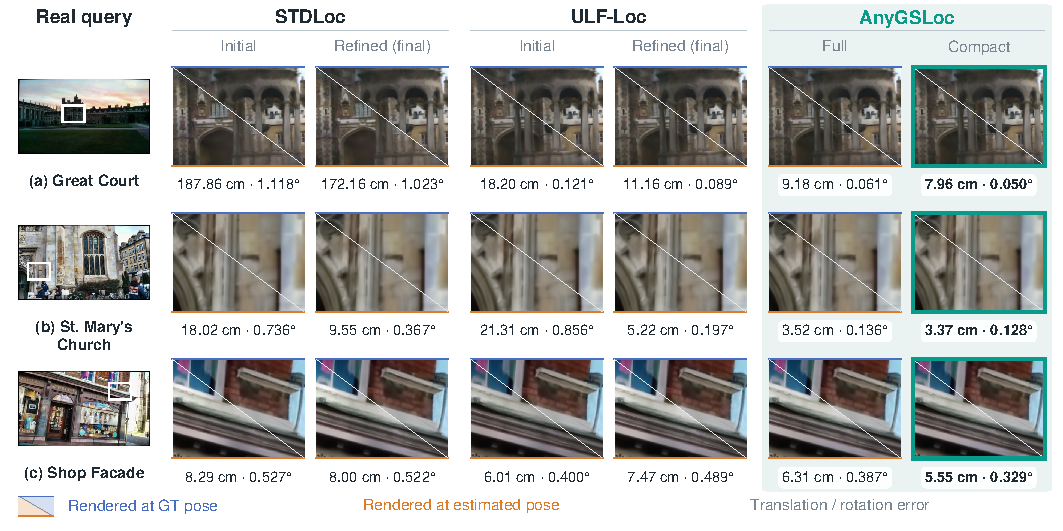
\includegraphics[width=\linewidth]{E1_final_localization.pdf}
\caption{Localization examples under Table~\ref{tab:t4}. Baselines show initial and refined poses; AnyGSLoc shows Full and Compact. Each crop combines rendering at the ground-truth pose (upper triangle) and estimated pose (lower triangle), using one shared 3DGS model. Labels report TE/RE; the lowest TE in each row is outlined.}
\label{fig:e1}
\end{figure*}

\begin{figure}[!t]
\centering
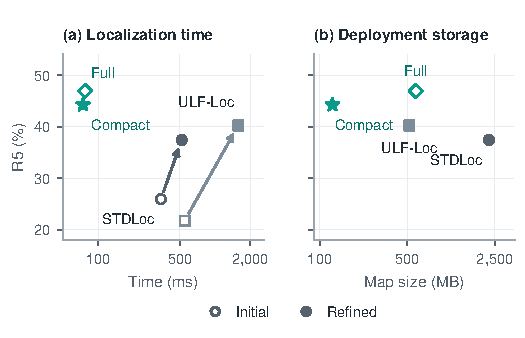
\includegraphics[width=\linewidth]{E5_deployment.pdf}
\caption{Accuracy and deployment cost on Cambridge (Table~\ref{tab:t4}). (a) Localization time; arrows connect baseline initialization and refinement. (b) Final accuracy versus map size. Cost axes are logarithmic; timing follows Sec.~\ref{sec:setup}.}
\label{fig:e5}
\end{figure}


The local comparison highlights a useful distinction between localization accuracy and the complexity of the deployed pipeline. Compact achieves 8.54\,cm median TE and 44.25\% R5 in a single pose-estimation stage (Table~\ref{tab:t4}). Its median TE is close to the refined outputs of STDLoc and ULF-Loc, which improve from 11.22 to 8.88\,cm and from 12.19 to 8.37\,cm, respectively. The Full reference reaches 7.82\,cm and the highest R5 in this comparison. Figure~\ref{fig:e1} shows representative query alignments.

The corresponding deployment cost is substantially smaller. Compact requires 74.19\,ms of localization time and 126.73\,MB of scene-specific storage, compared with 518.01\,ms and 2,251.31\,MB for refined STDLoc and 1,574.00\,ms and 519.65\,MB for refined ULF-Loc. Full requires 77.22\,ms and 585.69\,MB. The main benefit of selection is therefore the reduction in persistent map size; the measured localization time changes only modestly because feature extraction and robust pose estimation remain common to the compared map variants. Figure~\ref{fig:e5} summarizes these operating points.

Mean errors reveal why median accuracy alone is insufficient for this comparison. Full and Compact have mean TE/RE of 21.12\,cm/$0.236^\circ$ and 19.74\,cm/$0.238^\circ$, respectively. In contrast, STDLoc refinement improves its median and R5 while increasing mean TE/RE from 75.06\,cm/$1.078^\circ$ to 311.15\,cm/$1.384^\circ$. The mean and tail statistics therefore expose occasional large pose failures that are hidden by the median.

\subsection{Landmark Geometry and Appearance}
\label{sec:construction-results}
\begin{table}[!t]
\centering
\footnotesize
\setlength{\tabcolsep}{2pt}
\renewcommand{\arraystretch}{1.10}
\caption{Landmark coordinates with shared observations}\label{tab:t5}
\begin{tabular*}{\linewidth}{@{\extracolsep{\fill}}lcc@{}}
\toprule
Coordinate source & \shortstack{Median TE/RE\\(cm/deg)} & R5 (\%) \\
\midrule
\multicolumn{3}{l}{\textit{(a) Vanilla 3DGS}} \\
Gaussian centers & \underline{9.978}/\underline{0.141} & \underline{37.83} \\
Rendered depth & 94.831/0.878 & 8.04 \\
Multiview triangulation & \textbf{7.950}/\textbf{0.119} & \textbf{46.21} \\
\midrule
\multicolumn{3}{l}{\textit{(b) MAtCha}} \\
Gaussian centers & 10.509/\underline{0.149} & \underline{35.96} \\
Rendered depth & \underline{9.459}/0.153 & 31.12 \\
Multiview triangulation & \textbf{8.511}/\textbf{0.132} & \textbf{42.34} \\
\bottomrule
\end{tabular*}
\tabnote{Tracks, observations, descriptors, and query processing are fixed for each Gaussian model; selection is disabled. The 3DGS and MAtCha common pools contain 421,224 and 352,334 landmarks. Bold/underline: best/second-best within each Gaussian model.}
\end{table}

\begin{figure}[!t]
\centering
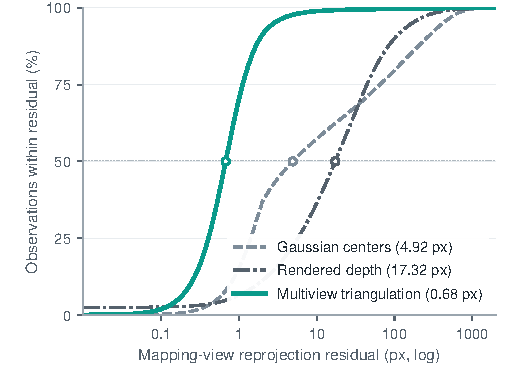
\includegraphics[width=\linewidth]{E2_geometry_source_evidence.pdf}
\caption{Mapping-view reprojection residuals for the 3DGS control: 1,346,981 shared observations of 116,303 landmarks in St.~Mary\textquotesingle s Church. Legend values are median residuals; invalid projections remain in the CDF denominator. Table~\ref{tab:t5} evaluates query-pose accuracy from the same coordinate sources.}
\label{fig:e2}
\end{figure}


\paragraph{Coordinate sources}
We first ask where the 3D coordinate of a localization landmark should come from. Table~\ref{tab:t5} holds the landmark identities, eligible observations, Full-map descriptors, and query processing fixed for each Gaussian model while disabling selection. Gaussian-center and rendered-depth alternatives are aggregated from the common observations, whereas the proposed coordinate is obtained by multiview ray triangulation. The resulting common pools contain 421,224 landmarks for vanilla 3DGS and 352,334 for MAtCha; these pools are used only for this controlled coordinate-source study.

The result directly supports the geometric design in Sec.~\ref{sec:geometry}. Triangulation gives the lowest median TE and highest R5 for both evaluated Gaussian models. On vanilla 3DGS, median TE is 7.95\,cm for triangulation, compared with 9.98\,cm for Gaussian centers and 94.83\,cm for rendered depth. On MAtCha, the corresponding values are 8.51, 10.51, and 9.46\,cm. The large variation of rendered-depth performance also shows that depth back-projection is tied to the depth behavior of the underlying scene representation. Figure~\ref{fig:e2} visualizes the reprojection discrepancy using shared 3DGS observations. This experiment isolates coordinate assignment; it does not measure error against an independently reconstructed ground-truth surface.

\begin{table}[!t]
\centering
\footnotesize
\setlength{\tabcolsep}{1.3pt}
\renewcommand{\arraystretch}{1.15}
\caption{Filtering and fusion on Compact maps}\label{tab:t6}
\begin{tabular*}{\linewidth}{@{\extracolsep{\fill}}ccccccc@{}}
\toprule
Filter & Fusion & \shortstack{Map\\points} & \shortstack{Med. TE/RE\\(cm/deg)} & \shortstack{Mean TE/RE\\(cm/deg)} & \shortstack{P95 TE\\(cm)} & R5 (\%) \\
\midrule
$\times$ & $\times$ & 116,020 & 8.792/0.124 & 20.438/0.267 & 55.759 & 41.51 \\
$\checkmark$ & $\times$ & 121,379 & 8.883/0.124 & \textbf{19.178}/\underline{0.258} & 54.814 & 41.59 \\
$\times$ & $\checkmark$ & 116,020 & \textbf{8.533}/\underline{0.122} & 21.244/0.283 & \underline{50.038} & \textbf{44.33} \\
$\checkmark$ & $\checkmark$ & 121,379 & \underline{8.537}/\textbf{0.121} & \underline{19.740}/\textbf{0.238} & \textbf{45.691} & \underline{44.25} \\
\bottomrule
\end{tabular*}
\tabnote{Within each filtering condition, fusion changes only descriptors; selected IDs and coordinates are identical. Single descriptors use fixed lexicographic order. Map sizes follow the same adaptive selector. Bold/underline: best/second-best among the four configurations.}
\end{table}


\paragraph{Observation filtering and descriptor fusion}
Table~\ref{tab:t6} evaluates the two appearance-side components together because they act at different points in the construction pipeline. Observation filtering changes which detections enter association, whereas descriptor fusion changes how the observations of an established track are represented. For each condition, the single-descriptor and fused variants use the same selected coordinates and landmark identities; the single descriptor is the first observation in a fixed lexicographic order. Because filtering changes the candidate graph, the selector can produce different natural map sizes.

The two mechanisms show complementary effects. Descriptor fusion increases R5 by 2.82 percentage points without filtering and by 2.66 points with filtering, and lowers both median and P95 TE in the corresponding comparisons. Observation filtering has a smaller effect on the median but reduces the error tail of the fused map: P95 TE falls from 50.04 to 45.69\,cm, while mean TE/RE falls from 21.24\,cm/$0.283^\circ$ to 19.74\,cm/$0.238^\circ$. The experiment therefore supports the intended division of labor: fusion strengthens the representation available to matching, while filtering removes unreliable observations before they can influence track construction.

\subsection{Map Compression and Localization Accuracy}
\label{sec:selection-results}
\begin{table}[!t]
\centering
\footnotesize
\setlength{\tabcolsep}{1.5pt}
\renewcommand{\arraystretch}{1.15}
\caption{Landmark selection and equal-budget alternatives}\label{tab:t7}
\begin{tabular*}{\linewidth}{@{\extracolsep{\fill}}lcccc@{}}
\toprule
Selection & Points & \shortstack{Med. TE/RE\\(cm/deg)} & \shortstack{P95 TE\\(cm)} & R15 (\%) \\
\midrule
Full & 560,996 & 7.817/0.117 & 43.907 & 74.54 \\
\midrule
\multicolumn{5}{@{}l}{\textit{(a) Selection stages}} \\
Q & 96,256 & 8.997/\underline{0.123} & 57.900 & 71.68 \\
Q+C & 103,274 & \underline{8.931}/\underline{0.123} & \underline{55.829} & \underline{72.15} \\
Q+C+P (Compact) & 121,379 & \textbf{8.537}/\textbf{0.121} & \textbf{45.691} & \textbf{73.12} \\
\midrule
\multicolumn{5}{@{}l}{\textit{(b) Same per-scene landmark budget}} \\
Spatial sampling & 121,379 & 14.222/0.197 & 95.939 & 59.04 \\
Quality Top-$K$ & 121,379 & \underline{8.729}/\textbf{0.119} & 56.497 & \underline{71.99} \\
Track-length Top-$K$ & 121,379 & 9.144/0.124 & \underline{49.582} & 71.93 \\
Q+C+P (Compact) & 121,379 & \textbf{8.537}/\underline{0.121} & \textbf{45.691} & \textbf{73.12} \\
\bottomrule
\end{tabular*}
\tabnote{Q: quality pruning; C: coverage completion; P: pose-aware completion including cleanup. Full is the reference before selection. Compact is repeated in (b) for direct comparison. Bold/underline: best/second-best within each block; point counts are not ranked.}
\end{table}

\begin{figure*}[!t]
\centering
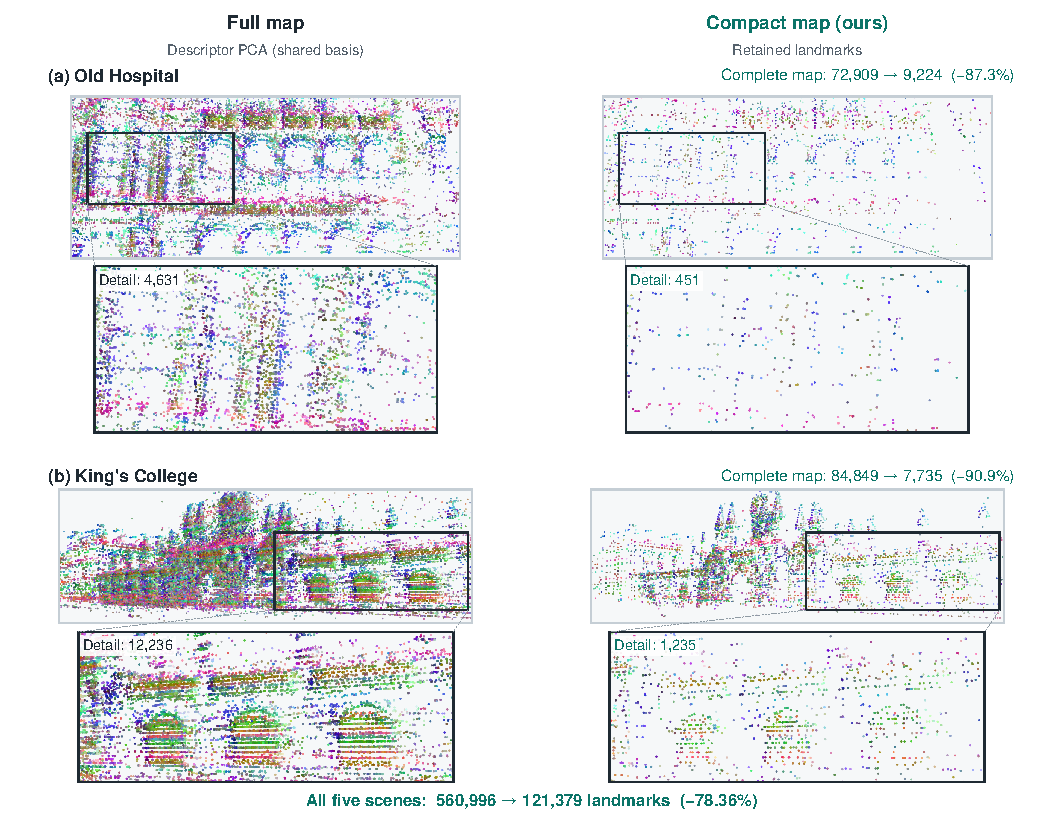
\includegraphics[width=\linewidth]{E3_compact_map.pdf}
\caption{Full and Compact maps from identical cameras and detail crops. A shared descriptor-PCA transform preserves colors for retained landmarks; Compact shows only selected points. Complete-map counts and cropped-region counts are distinguished. Across five scenes, selection removes 78.36\% of the 560,996 landmarks.}
\label{fig:e3}
\end{figure*}


Selection is evaluated next at the level of the deployed map. Compact retains 121,379 of the Full map's 560,996 landmarks, removing 78.36\% of the points (Fig.~\ref{fig:e3}). Storage decreases from 585.69 to 126.73\,MB, while average scene-median TE changes from 7.82 to 8.54\,cm and R15 from 74.54\% to 73.12\%. The important observation is that the reduction is not obtained by uniformly discarding useful structure: the selected map preserves most of the localization performance while removing a large fraction of the stored representation.

Table~\ref{tab:t7}(a) shows how the selection stages contribute to this behavior. Quality pruning alone gives 9.00\,cm median TE. Coverage completion reduces it to 8.93\,cm, and the final pose-aware stage reaches 8.54\,cm. More importantly, P95 TE decreases from 57.90 to 55.83 and then to 45.69\,cm. The final stage therefore contributes information beyond simply restoring the number of features visible in each reference view; its additions are chosen relative to the pose constraints already supplied by the map, followed by the support-preserving cleanup described in Sec.~\ref{sec:selection}.

Table~\ref{tab:t7}(b) compares the final selector with simpler alternatives. Compact achieves the lowest median TE and P95 TE and the highest R15 among the listed selectors. Quality Top-K and track-length Top-K reach 8.73 and 9.14\,cm median TE, respectively. Quality Top-K has slightly higher R5 (46.08\% versus 44.25\%), whereas track-length Top-K has lower mean TE (15.71 versus 19.74\,cm). The comparison is consequently not a claim that every individual metric is maximized by Compact; rather, it shows that combining quality, coverage, and conditional pose information yields a balanced operating point after substantial map reduction.

\subsection{Compatibility Across Gaussian Representations}
\label{sec:priors}
\begin{table}[!t]
\centering
\footnotesize
\setlength{\tabcolsep}{1.7pt}
\renewcommand{\arraystretch}{1.15}
\caption{Compact maps from different Gaussian models}\label{tab:t8}
\begin{tabular*}{\linewidth}{@{\extracolsep{\fill}}lcccc@{}}
\toprule
Gaussian model & \shortstack{PSNR\\(dB)} & \shortstack{Med. TE/RE\\(cm/deg)} & R5 (\%) & \shortstack{Map\\(MB)} \\
\midrule
Vanilla 3DGS & \textbf{16.72} & \textbf{8.537}/\textbf{0.121} & \textbf{44.25} & \textbf{126.73} \\
MAtCha & 15.46 & \underline{8.844}/0.132 & \underline{42.07} & \underline{196.28} \\
Vanilla 2DGS & \underline{15.70} & 8.922/\underline{0.127} & 39.95 & 196.84 \\
i3DGS raw & 13.66 & 22.904/0.384 & 11.77 & 351.27 \\
i3DGS post-opt. & 15.14 & 10.858/0.175 & 30.29 & 244.58 \\
Long-LRM raw & 13.56 & 483.413/7.344 & 11.25 & 315.00 \\
Long-LRM post-opt. & 15.34 & 147.566/3.178 & 22.50 & 261.27 \\
\bottomrule
\end{tabular*}
\tabnote{PSNR uses mapping views. Post-opt.: 1,000 upstream updates. All input models use the same downstream pipeline with natural map sizes; native reconstruction settings differ. Bold/underline: best/second-best.}
\end{table}

\begin{figure*}[!t]
\centering
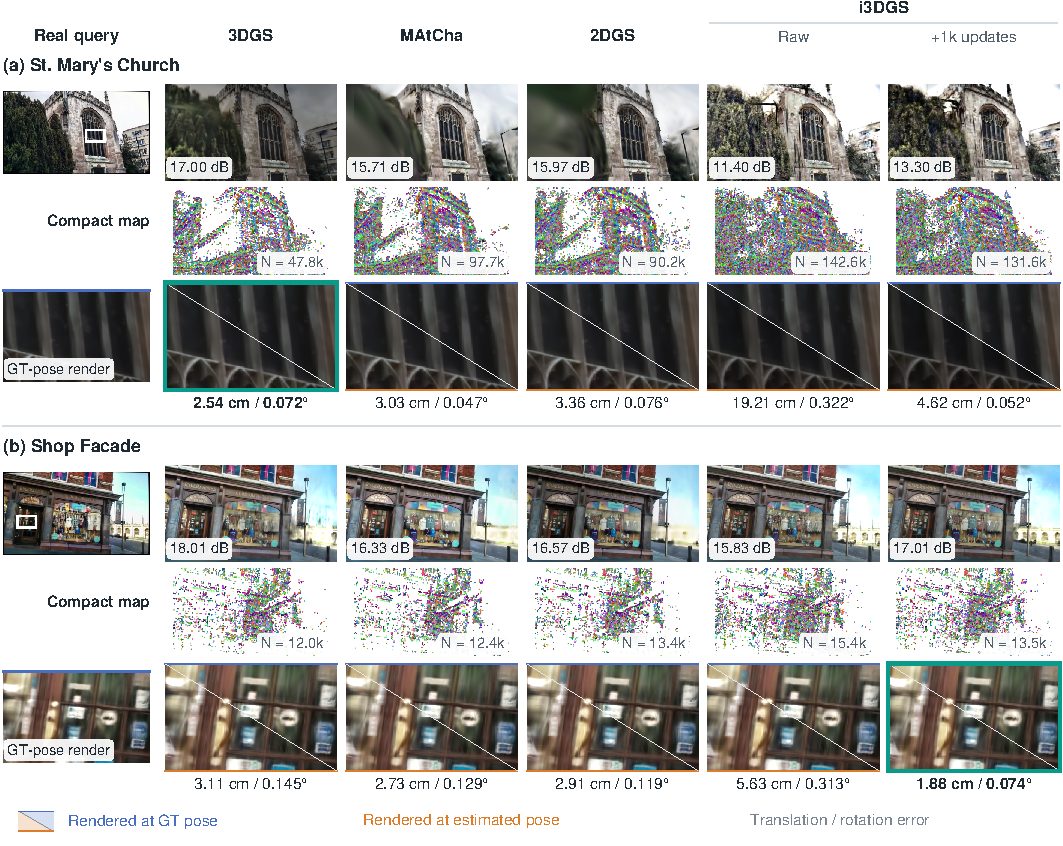
\includegraphics[width=\linewidth]{E4_gaussian_prior.pdf}
\caption{Compact maps from different Gaussian models (Table~\ref{tab:t8}). Top: reference-view renderings, with scene-average reference PSNR. Middle: map geometry and complete point counts. Bottom: pose alignment using a shared 3DGS renderer and the diagonal convention of Fig.~\ref{fig:e1}. Post-optimized i3DGS uses 1,000 upstream updates.}
\label{fig:e4}
\end{figure*}


A useful conversion method should not depend on one particular Gaussian training pipeline. Table~\ref{tab:t8} applies the same downstream construction and selection procedure to seven input conditions, including vanilla 3DGS, MAtCha, vanilla 2DGS, incremental i3DGS~\cite{meuleman2026i3dgs}, and feed-forward Long-LRM~\cite{chen2025longlrm}, with the latter two evaluated before and after 1,000 upstream optimization steps. Native upstream settings are retained; only the downstream conversion to an explicit landmark map is shared.

Vanilla 3DGS, MAtCha, and vanilla 2DGS produce similar median TE of 8.54, 8.84, and 8.92\,cm, respectively. For the less mature input reconstructions, upstream optimization substantially changes localization quality: i3DGS improves from 22.90 to 10.86\,cm and Long-LRM from 483.41 to 147.57\,cm. These results support compatibility with different Gaussian representations while making the dependence on input observation quality explicit.

Rendered-image quality alone is not a sufficient predictor of localization quality. Post-optimized Long-LRM has slightly higher mapping-view PSNR than i3DGS (15.34 versus 15.14\,dB), yet its localization error is much larger. Figure~\ref{fig:e4} provides representative renderings, reconstructed maps, and query alignments. The comparison supports using localization measurements, rather than image-reconstruction quality alone, to judge the suitability of a Gaussian scene as an input to map construction.

\subsection{Optional Use of Mapping Images}
\label{sec:input-availability}
\begin{table}[!t]
\centering
\footnotesize
\setlength{\tabcolsep}{3pt}
\renewcommand{\arraystretch}{1.10}
\caption{Availability of original mapping images}\label{tab:t9}
\begin{tabular}{@{}lccc@{}}
\toprule
Observations & \shortstack{Median TE/RE\\(cm/deg)} & R5 (\%) & Map (MB) \\
\midrule
\multicolumn{4}{@{}l}{\textit{Full}} \\
Gaussian renderings & 7.817/\underline{0.117} & \underline{46.95} & \underline{585.69} \\
Reference images & \underline{7.249}/0.124 & 43.94 & \textbf{550.22} \\
Both & \textbf{6.567}/\textbf{0.107} & \textbf{47.52} & 589.70 \\
\midrule
\multicolumn{4}{@{}l}{\textit{Compact}} \\
Gaussian renderings & 8.537/\underline{0.121} & \underline{44.25} & \textbf{126.73} \\
Reference images & \textbf{7.706}/0.123 & 42.31 & 358.08 \\
Both & \underline{8.282}/\textbf{0.119} & \textbf{45.40} & \underline{163.95} \\
\bottomrule
\end{tabular}
\tabnote{Each source condition has a 2,048-feature budget per reference view; Both splits it equally. Map sizes are natural outcomes of the same selector. Bold/underline: best/second-best within each map variant.}
\end{table}


Original mapping images can provide additional observations when they are available, but they are not required by the default conversion. Table~\ref{tab:t9} compares the rendering-only default with an image-only reference and a combined input. The rendering-only and image-only conditions use up to 2,048 features per reference view; the image-only condition does not use Gaussian-dependent filtering or depth augmentation. The combined condition uses 1,024 features from each source and applies observation filtering to both. All conditions share the same query processing and adaptive map selector, with the reported map sizes arising naturally from the available observations.

Adding original images improves the Compact median TE from 8.54 to 8.28\,cm and R5 from 44.25\% to 45.40\%, at the cost of increasing storage from 126.73 to 163.95\,MB. Image-only maps reach 7.71\,cm but require 358.08\,MB. The Full map also benefits from the additional observations, reaching 6.57\,cm and 47.52\% R5. This experiment treats original images as an optional source of additional evidence rather than as a requirement of the framework.

\subsection{Limitations}
\label{sec:limitations}

The resulting map remains dependent on the quality and coverage of the reference observations. Rendering errors that are consistent across views can survive the observation checks and enter a track, while a single fused descriptor may be insufficient for large appearance changes. The selection criteria are derived from reference-view support and local pose information; their benefit therefore depends on how well the selected views represent the eventual query distribution. Finally, the evaluation targets known-scene single-image relocalization. Very large environments may require retrieval or spatial partitioning, and changing environments would require map maintenance beyond the present offline construction setting.
\section{Conclusion}
\label{sec:conclusion}

AnyGSLoc converts a prebuilt Gaussian scene into an explicit localization map whose landmarks are grounded in multiview feature correspondences rather than in the identities of rendering primitives. Gaussian rendering supplies the offline observations and geometric cues; feature tracks determine the exported 3D coordinates and descriptors, and localization-aware selection reduces the map to the landmarks most useful for deployment. The resulting map supports direct 2D--3D localization without accessing the Gaussian renderer online.

Across 24 indoor and outdoor scenes, the Compact map achieves 8.54\,cm/$0.12^\circ$ average scene-median error on Cambridge, with 126.73\,MB of scene-specific storage. Relative to the Full candidate bank, it removes 78.36\% of the landmarks and reduces storage from 585.69 to 126.73\,MB while increasing average scene-median translation error from 7.82 to 8.54\,cm. Controlled studies further support multiview triangulation as the coordinate source and show complementary effects of observation filtering and descriptor fusion. These results indicate that a renderable Gaussian scene can serve as a practical source for a compact, correspondence-based localization map without making the rendering representation itself part of the deployed localizer.
\IEEEtriggeratref{47}
\bibliographystyle{IEEEtran}
\bibliography{references,reported_references,related_references}
\end{document}